\section{Noise Reduction}
\label{sec:noise-reduction}

The method of \emph{Canny edge detection} is solely based on gradients, and the gradient calculation is very sensitive to noise. So, it is necessary to reduce noise in the image before applying the edge detection algorithm. There are several methods to reduce noise in an image. The most common method is to apply a \emph{Gaussian filter} to the image. It is a low-pass filter that removes high-frequency noise from the image; i.e., it smoothens the image.

\begin{equation}
    \label{eq:gaussian-filter}
    H(x, y) = \frac{1}{2\pi\sigma^2}e^{-\frac{x^2 + y^2}{2\sigma^2}}
\end{equation}

Where, $H(x, y)$ is the Gaussian filter, $\sigma$ is the standard deviation of the Gaussian distribution, and $x$ and $y$ are the coordinates of the filter. The Gaussian filter is applied to the image using convolution.

After applying the Gaussian filter, the image becomes less noisy, and the edges become more pronounced. This is illustrated in \autoref{fig:noise-reduction}.

\begin{figure}[ht]
    \centering
    \begin{subfigure}[b]{0.4\textwidth}
        \centering
        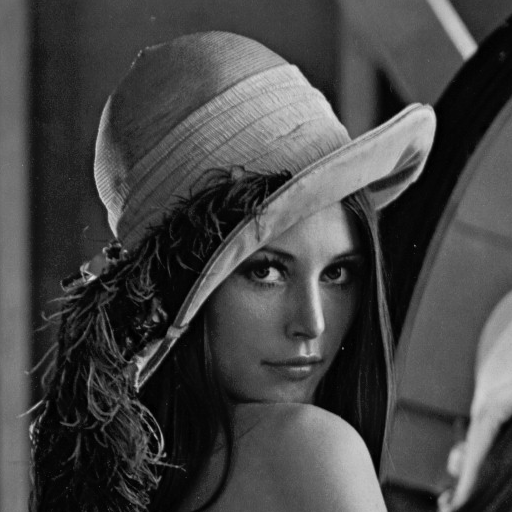
\includegraphics[width=0.9\textwidth]{lenna_2_grayscale.png}
        \caption{Original Grayscale Image}
        \label{fig:grayscale-original}
    \end{subfigure}
    \hfill
    \begin{subfigure}[b]{0.4\textwidth}
        \centering
        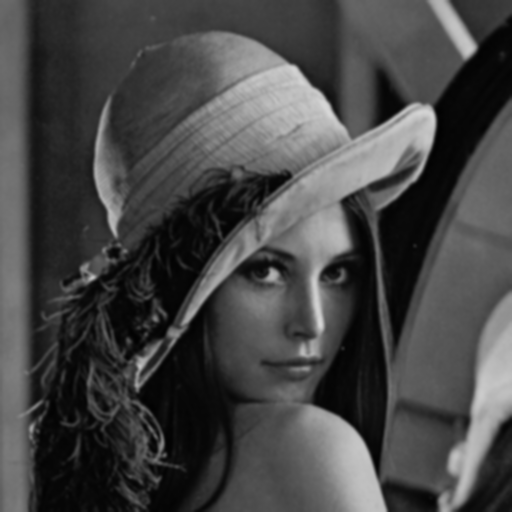
\includegraphics[width=0.9\textwidth]{lenna_3_blurred.png}
        \caption{Image after Applying Gaussian Filter ($5\times5$)}
        \label{fig:gaussian-filter}
    \end{subfigure}
    \caption{Effect of Noise Reduction on an Image}
    \label{fig:noise-reduction}
\end{figure}